\documentclass[10pt]{article}
\usepackage[polish]{babel}
\usepackage[utf8]{inputenc}
\usepackage[T1]{fontenc}
\usepackage{amsmath}
\usepackage{amsfonts}
\usepackage{amssymb}
\usepackage[version=4]{mhchem}
\usepackage{stmaryrd}
\usepackage{graphicx}
\usepackage[export]{adjustbox}
\graphicspath{ {./images/} }

\title{LIGA MATEMATYCZNA im. Zdzisława Matuskiego \\
 FINAE \\
 16 kwietnia 2018 \\
 SZKOŁA PODSTAWOWA \\
 (klasy IV - VI) }

\author{}
\date{}


\begin{document}
\maketitle
\section*{ZADANIE 1.}
W rodzinie Bartka są cztery osoby. Suma ich lat jest równa 100. Bartek jest o 4 lata starszy od Ani, a tata jest o 6 lat starszy od mamy. Ania poprosiła złotą rybkę, aby cofnęła czas o całkowitą liczbę lat do momentu, w którym Ania była sześć razy młodsza od mamy. Złota rybka zastanowiła się i cofnęła czas o pięć lat. Ile lat mają członkowie rodziny po cofnięciu czasu?

\section*{ZADANIE 2.}
Podaj wszystkie liczby trzycyfrowe o sumie cyfr równej 9 i cyfrze setek podzielnej przez 4.

\section*{ZADANIE 3.}
Sierżant przygotowywał oddział żołnierzy do defilady. Próbował ustawiać ich trójkami, ale jeden żołnierz pozostawał. Także po ustawieniu czwórkami, piątkami i szóstkami jeden żołnierz zostawał. W końcu ustawił ich siódemkami i wtedy siódemki były kompletne. Jaka mogła być najmniejsza liczba żołnierzy w tym oddziale?

\section*{ZADANIE 4.}
Wykaż, że liczba \(10^{20}+19^{3}-2\) jest podzielna przez 9 .

\section*{ZADANIE 5.}
Punkt \(S\) jest środkiem okręgu opisanego na trójkącie ostrokątnym \(A B C\). Miara kąta \(A C S\) jest trzy razy większa od miary kąta \(B A S\), a miara kąta \(C B S\) jest dwa razy większa od miary kąta \(B A S\). Wyznacz miary kątów trójkąta \(A B C\).\\
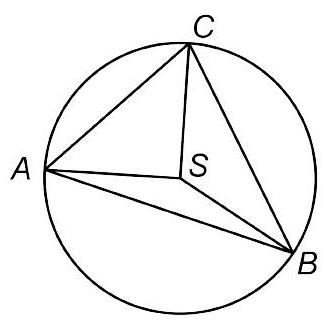
\includegraphics[max width=\textwidth, center]{2024_11_21_bf918c4f5acb20cb8c1bg-1}


\end{document}